% ========================
% # Administração        #
% ========================

\section{Administração}

\subsection{Introdução}

O Pelouro da Administração não dá apenas apoio aos outros pelouros nem trata só de gerir o Núcleo. Exemplo disso, é o vasto leque de atividades realizadas por este Pelouro que, ao longo do ano, contou com a renovação dos espaços de estudo do Departamento, salas de estudo do piso 6, piso 4 e piso 3, que outrora não tinham grandes condições para o efeito. Para além disso, como atividades, esta equipa organizou os jantares de curso dos dois semestres e várias febradas e cachorradas, que acompanharam eventos de outros pelouros, para além do apoio logístico das atividades e da devida administração do Núcleo já referida no Relatório de Mandato e referida no Inventário.

\subsection{Atividades}

% =================================
% # Arranjo dos Espaços de Estudo #
% =================================

\subsubsection{Arranjo dos Espaços de Estudo}

Ao longo dos últimos têm existido inúmeras queixas, fundamentadas, pela falta de condições nos espaços de estudo do \acrshort{deec}. Apesar de existirem vários espaços abertos 24 horas (as varandas do piso 3, a sala de estudo do piso 6 e a sala T.4.2, para além da sala T.4.3, antes da criação do \acrlong{cp}), estes espaços não dispunham de tomadas elétricas e internet e tinham o seu espaço completamente desorganizado havendo faltas de cadeiras, etc. No sentido de lutar para que houvessem espaços de estudo com qualidade para os nossos estudantes, este ano, decidimos meter mãos à obra, falar com a Direção do \acrshort{deec} e renovar completamente os espaços já existentes, pondo de parte a inércia da Manutenção do Departamento.

Começamos com o arranjo do piso 3, um espaço bastante usado durante o dia, mas que apresentava vários problemas, como falta de pontos de eletricidade e lâmpadas e cadeiras que faziam muito barulho quando arrastadas ou outras que não existiam.

Inicialmente fizemos novas montagens elétricas nas divisórias, de modo a ter um interruptor maior e mais resistente que o anterior, de forma a que não fosse fácil que este se partisse, mesmo com o uso, como acontecia com os anteriores. A seguir afixamos extensões às laterais das divisórias, ficando cada lado das mesmas com 3 pontos de eletricidade, ou seja 6 pontos por cada 4 pessoas.

Após essa instalação, mudamos todas as cadeiras de forma a uniformizar o layout do espaço e a garantir que todos os lugares dispunham de uma cadeira. No total, este espaço, ficou com 40 lugares disponíveis.

Ficou um espaço muito bom para estudar sendo, no entanto, frio durante o Inverno mas infelizmente este é um problema que não tem resolução aparente dadas as condições do edifício.

Passamos à renovação da Biblioteca do Piso 6, onde o problema era outro, completamente diferente, o barulho, aliado à desorganização.

Numa fase inicial, ainda no verão, começámos por fazer um mapa da sala e criámos uma fila de mesas junto à parede e a respetiva eletrificação, através de calha, garantindo 3 pontos de luz para cada 2 lugares. Também no verão, rompemos com o contrato da máquina de vending, tendo a mesma sido removida.

Em outubro, mudamos o layout da sala:
\begin{itemize}
\item Parte de estudo em grupo – Antes do vidro.
\item Parte de estudo individual – Após o vidro.
\end{itemize}

Na parte de estudo em grupo agrupamos pares de mesas ficando um total de 5 grupos de mesas, ou seja, 20 lugares ao todo, nesta parte, com extensões elétricas para todos.

Na parte de estudo individual encostámos uma fila de mesas à parede, de uma ponta à outra da sala, e colocando uma calha ao longo de toda essa fila, proporcionando 3 pontos de eletricidade para cada 2 pessoas. No meio da sala colocamos 2 filas de mesas frente a frente nas quais ficou a faltar a implementação da última fase do projeto.

No total ficamos com cerca de 80 lugares nesta parte totalizando 43\% mais lugares em toda a sala que anteriormente.

Passado alguns meses, em março, após a chegada das divisórias compradas pelo \acrshort{neeec} e pagas pelo \acrshort{deec}, procedemos à fase final da renovação, na qual colocamos as divisórias entre as 2 filas de mesas do centro. Depois da colocação destas afixámos extensões em cada divisória, ficando com o mesmo rácio, de tomadas por pessoa, que as mesas da parede.

Pedimos ao \acrshort{gri} para implementar “lag” e bloquear jogos na rede de Internet da biblioteca, de forma a que as pessoas usassem a sala para estudo e não para fins lúdicos (que ajudam a criar barulho) contudo, após a UGF, esta implementação caiu.

A ideia das divisórias surgiu como forma de diminuir o barulho, para que as pessoas não falassem com a pessoa em frente. Este problema melhorou de facto mas existem momentos em que continua a verificar-se barulho na sala e a solução não parece estar à vista, visto que mesmo tentando sensibilizar as pessoas a fazerem silêncio o problema persiste. Contudo, sempre que alguém manda calar os restantes a sala fica em silêncio absoluto acabando por ter menos barulho quando está cheia do que quando está "a meio".

Na sala de estudo T.4.2 tirámos as mesas cinzentas que lá estavam e pusemo-las no arrumo B1, uniformizando o design do espaço, apenas com mesas e cadeiras de madeira. Prendemos as mesas que estavam encostadas à parede à mesma e as restantes entre si. Adicionalmente, colocámos um mapa da disposição correta da sala para que sempre que haja eventos a sala seja colocada de forma correta. No total ficamos com 32 lugares nesta sala tendo a mesma sido também alvo de eletrificação e arranjos pontuais como o facto de se ter prendido o quadro e as luzes e substituídas as lâmpadas fundidas do teto.

Quer na sala T.4.2 como nas varandas do Piso 3 é muito comum os estudantes fumarem nos jardins anexos e, não tendo local onde se sentar, levam as cadeiras de madeira para a rua fazendo com que estas se estraguem e deixem de haver cadeiras em todos os lugares. De forma bem sucedida, para prevenir isto, colocámos cadeiras de plástico, próprias para rua, em todos os locais de fumo.

Em todos os espaços de estudo foram colocados avisos que incentivam ao silêncio, ao fecho das luzes, ao facto de não se dever jogar naqueles locais e publicidade à plataforma de queixas logísticas do \acrshort{neeec}. Estes avisos foram colocados em todos os locais de estudo (1 aviso para cada 2 lugares) tendo sido um sucesso, dado a sua componente mais amiga.


\ifthenelse{\boolean{biblia}}
{ % TRUE
	% =================================
% # Cachorrada da Tomada de Posse #
% =================================

\subsubsection{Cachorrada da Tomada de Posse}
\label{subseccachorradaTomadaPosse}

Após a tomada de posse propriamente dita, passou-se aos festejos da mesma, proporcionando a todos os presentes uma cachorrada com finos.

Esta cachorrada tinha entrada paga e dava acesso livre a cachorros, finos e sumos de laranja. O evento era aberto à comunidade do \acrshort{deec} e do \acrshort{dei}. As pulseiras utilizadas eram de um Mega Convívio anterior pelo que foram detetadas duas entradas falsificadas derivadas do facto de todos os núcleos do Polo 2 terem um arquivo desse tipo de pulseiras. O facto de poder haver pessoas sem pulseira na zona fez também com que houvesse um controlo mais difícil de quem comia ou não. Contudo, todas as situações deste tipo, que foram detetadas, foram excecionais e não puseram em causa a sustentabilidade do evento pelo que, para evitar confusões, nem foram divulgadas. Ao início da noite, houve também vários elementos da Direção Cessante que queriam que o serviço da comida fosse livre mas tal não foi permitido para evitar demasiada confusão. Contudo, no decorrer da noite, o serviço passou a ser feito por quem queria algo, quando já não havia confusão nenhuma com filas.

Esta só começou após a tomada de posse do \acrshort{nei} terminar, ou seja, houve tempo para montar tudo quanto antes, nos jardins do \acrshort{neeec}.

No decorrer do evento, apesar de terem sido feitas as compras antes, foi necessário ir ao continente, de urgência, comprar mais pão de cachorro. Em termos logísticos foi um evento relativamente fácil de organizar, sendo só necessário pedir uma botija de gás e um fogão ao \acrshort{nei}, organizar mesas e pedir a máquina de finos e o barril. Em relação à comida foi necessário comprar latas de salsichas, pão de cachorro, molhos e guardanapos.
    
	% ========================
% # Febrada IEEE         #
% ========================

\subsubsection{Febrada de Apresentação do IEEE}

No dia 23 do mês de novembro foi realizada uma febrada em conjunto com o \acrfull{ieeeuc}. O local inicialmente escolhido para tal foram as escadas em frente à entrada do \acrshort{deec} tendo sido alterado mais tarde, devido à probabilidade de chuva, para junto do estacionamento de bicicletas/motas entre o \acrshort{deec} e o \acrshort{dei}.

Foi usada uma tenda junto ao pequeno telheiro existente, onde se colocou a máquina de finos, mesas para servir e logo a seguir a mesa da caixa para se efetuar a compra de senhas. O grelhador ficou na parte de trás com uma mesa de apoio.
No inicio da febrada foi ainda necessário a colocação de mais uma mesa e duas cadeiras para promover um ginásio com descontos para estudantes.

Em termos logísticos não foi difícil de organizar o evento. A parte mais complicada foi o preenchimento da escala, e o facto de já no decorrer da febrada ser necessário a colocação da mesa extra, o fez com que fosse necessário recorrer a pessoas não escaladas. 

O evento não teve muita adesão, onde o tempo pode ser uma das principais razões para isso.

De notar que esta febrada tinha como propósito promover o \acrshort{ieeeuc}, à semelhança do que se fez no ano anterior, mas a equipa desta entidade não se promoveu de forma alguma tendo este propósito caído por terra.

\ifthenelse{\boolean{biblia}}
{ % TRUE
	Este evento só teve um saldo positivo uma vez que o único barril utilizado foi vendido, ainda a meio, a um Carro da Queima das Fitas de Engenharia Biomédica e não foi cobrado pela \acrshort{dg}. Caso contrário, este evento teria dado prejuízo.
}
{ % FALSE
}


    
	% ===============================
% # Jantares de Curso           #
% ===============================

\subsubsection{Jantares de Curso}

Os Jantares de Curso são a maior atividade de convívio de todos os estudantes do \acrshort{deec}, por razões bastante óbvias. Normalmente é o Núcleo que organiza os primeiros jantares de cada semestre e os carros organizam os jantares da serenata da Latada e da Queima das Fitas.

Este ano a Latada foi adiantada uma semana, fazendo com que não existisse jantar de serenata, uma vez que se tinha feito jantar de curso uma semana antes e seriam já demasiados jantares num curto espaço de tempo. Para além disso, deixou de haver febrada dos carros antes do Mega-Convívio, portanto o Núcleo achou por bem deixar dividir o jantar com os carros, ao abrigo de um contrato.

O acordo estipulado entre o Núcleo e os Carros contemplava não só a divisão de tarefas, como também, a divisão do lucro e eventuais multas/reduções de lucro.
As tarefas ficaram distribuídas da seguinte forma:
\begin{enumerate}
\item Contactar o local do jantar – Carro do Pedro Marçal
\item Fazer o cartaz e divulgar o evento – Carro da Carlos Abegão
\item Fazer a escala e verificar o cumprimento da mesma – \acrshort{neeec}
\item Controlar as entradas no jantar – \acrshort{neeec}
\end{enumerate}

Para ser justo para todos, caso existissem faltas à escala, a entidade responsável pela pessoa que faltou veria a sua percentagem de lucros reduzida em 1\% e esta seria distribuída equitativamente pelas restantes entidades. Caso existisse uma falta coberta por outro membro da entidade a percentagem seria reduzida em 0,5\%. Esta última medida foi implementada tendo em conta que havia muitas membros de um dos carros que pertenciam também ao Núcleo, representando as duas entidades.

O jantar foi no pavilhão da Palmeira e não correu como o esperado. Basicamente se quiséssemos encher o jarro tínhamos de ir à banca para que os empregados nos enchessem a mesma. O mesmo se aplicava aos finos, em que só se podia pedir 2 de cada vez.
Quanto ao serviço faltou comida a várias pessoas e o pavilhão não tinha as condições que um restaurante dispõe. Não obstante, o ambiente foi bom e correu tudo bem, com exceção de uma cadeira partida por um aluno, que nem se apercebeu de tal, e a organização teve de pagar imediatamente, algo que não é costume noutros locais até porque a mobília utilizada era de fraca qualidade.

O jantar do 2º semestre foi por conta do Núcleo, em exclusivo, portanto deu menos dores de cabeça. Fez-se uma banca no bar para as inscrições, com uma folha de registo de todo o dinheiro que entrava e saía da caixa. No entanto, houve alguns problemas com o dinheiro uma vez que havia inscrições pagas na banca do bar e outras pagas no núcleo e as pessoas não entendiam a necessidade de separar os registos de ambas as caixas.
O local escolhido foi o Restaurante da Torre do Arnado e no geral correu bastante bem, tirando o facto de que tínhamos marcado o local para 130 pessoas e só se inscreveram 88, o que já é hábito nos jantares do 2º semestre, que têm bastante menos adesão. Uma vez que houve um erro na observação do excel, informou-se a senhora do restaurante, no dia, que estavam inscritas 120 pessoas pelo que no ato de pagamento, a senhora cobrou 10€ dado o enorme rombo de clientes versus a quantidade de comida comprada e empregados contratados para o serviço. Assim este jantar deu um lucro reduzido novamente.

Recomendamos a manutenção destes jantares dado serem uma atividade tradicional. Contudo, aconselhamos a uma gestão melhor dos eventos de forma a que possam ter uma saldo mais positivo e um custo mais reduzido para os participantes.


    
	% ========================
% # Manual de Febradas   #
% ========================

\subsubsection{Manual de Febradas}

Fazer uma febrada parece a coisa mais simples do mundo e a verdade é que não é algo muito difícil. No entanto, falham sempre vários pequenos pormenores no decorrer das febras que são cruciais para o seu sucesso como, entre vários casos, por exemplo a falta de carvão no início das febradas, hora que costuma culminar com a saída das pessoas das aulas e, como tal, com a hora de maior afluência onde é fulcral ter o maior número de febras prontas para vender e garantir que a febrada tem retorno.

Assim, serve o presente guião para colmatar todas as possíveis falhas que possam ocorrer na preparação de uma febrada.

\paragraph{O que é necessário?}
Antes de mais, é preciso que exista um espaço para realizar o evento, daí ser necessário fazer o pedido de autorização de espaço. Para isso basta enviar um e-mail ao Diretor do Departamento com todas as informações do evento (data, hora e motivo), fazendo sempre referência ao comprometimento em deixar o espaço limpo e arrumado.

Posto isto é necessário fazer a “To-Do List”:
\begin{itemize}
    \item Compras
    \begin{itemize}
        \item Pão: a encomenda é feita normalmente na Padaria do Alto de S. João (239 714 313), ao lado do Pingo Doce da Portela. O preço é de 8 cêntimos/pão sendo, no entanto, necessário mencionar que a encomenda é para o \acrshort{neeec} e não é passada fatura. É também possível fazer a encomenda junto da Padaria onde o Lourenço Moniz (919 803 120‬), ex-aluno do curso, trabalha sendo o preço também de 8 cêntimos/pão e existindo fatura.
        \item Carne: o  talho do Continente do Coimbra Shopping (239700125) costuma ter sempre os melhores preços na carne de porco, daí ser costume encomendar-se quase sempre a carne lá. NOTA: 1kg de carne são aproximadamente 10 febras, ou seja, por cada quilo de carne encomendam-se entre 9 a 11 pães.
        \item Cerveja: à encomenda de barris está sempre associada a respetiva máquina de finos, os copos de plástico e a botija de gás. Normalmente encomendam-se barris em excesso, uma vez que se podem devolver se não forem abertos. Há várias entidades que vendem barris, como é exemplo da \acrshort{aac}, através do preenchimento de um formulário e posterior aviso ao Administrador da \acrshort{aac}. No entanto, este método deixou de existir a meio do mandato, pelo que se teve de optar por contactar o Alexandre Mota (919 499 556). Podem também pedir barris ao armazém da Sagres, que embora seja ligeiramente mais cara tem um serviço de entrega com um funcionamento muito melhor. Basta fazer a encomenda e, por norma, esta é entregue no sítio, hora e data que combinarem. O pagamento é feito após a febrada, conforme o número de barris utilizados.
        \item Carvão: normalmente é comprado no café Batina, ao lado do Polo 2. O custo de cada saco grande é de 12€ e, novamente, não é passado recibo, sendo também necessário referir que a encomenda é feita pelo \acrshort{neeec}.
        \item Outras compras: guardanapos, sacos do lixo, acendalhas, temperos p/ carne.
\end{itemize}

    \item Material necessário para o local da febrada:
    \begin{itemize}
        \item Tenda
        \item Grelhador
        \item Fita cola (para prender os sacos do lixo e as tabelas de preço)
        \item Extensões (para ligar a máquina de finos)
        \item Caixa registadora
        \item Saldo de caixa inicial
        \item Tabelas de preços impressas
        \item Mesas e cadeiras
        \item Panela
        \item Garfo Grande
        \item Faca
    \end{itemize}

    \item Coisas essenciais fazer nos dias antes da febrada
    \begin{itemize}
        \item Escala: é fulcral fazer a escala da febrada para posterior publicação no Slack! Façam SPAM para a equipa preencher toda a escala de modo a que esta não tenha “buracos” e funcione tudo normalmente. Deixo um exemplo de uma escala em baixo.\\
        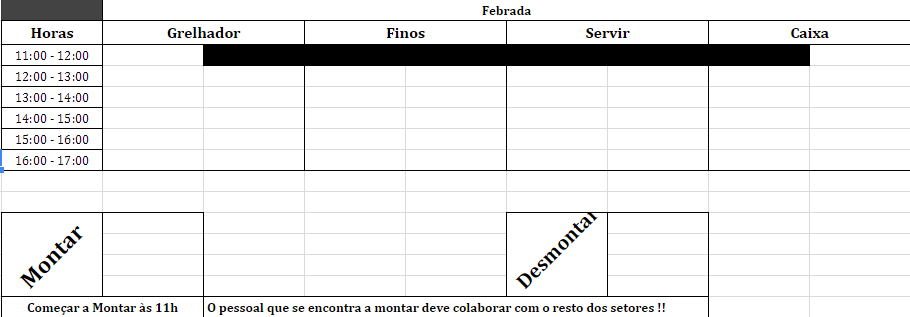
\includegraphics[width=0.88\textwidth]{imagens/escalas.png}
        \item Ligar a máquina de finos à corrente pelo menos um dia antes da febrada, para garantir que esta refresca.
        \item Pedir trocos ao Tesoureiro o quanto antes, para ter caixa inicial.
        \item Senhas e preçário: é essencial fazer senhas para cada evento específico, imprimi-las e cortá-las, bem como imprimir o preçário, que é discutido primeiro com o Tesoureiro. Não se esqueçam de rasgar e deitar as senhas ao lixo assim que as recebam durante a febrada para impedir as habituais borlas.
    \end{itemize}

    \item O dia da febrada
    \begin{itemize}
        \item Se forem seguidos todos os passos acima terão uma febrada de sucesso e neste dia só precisam de ir buscar as febras e o pão entretanto encomendados, montar a tenda e temperar as febras.
        \item Tempero das febras: juntem toda a carne num alguidar e deitem bastante massa de alho, pimentão doce, ervas de Provence, pimenta branca, sal e por fim, um fino. Usem luvas!
        \item É importante terem febras prontas antes da hora de afluência (meio-dia quando as mesmas são à hora de almoço), de modo a que não existam filas à hora de almoço e tudo flua super-rápido.
        \item No fim, deixem tudo limpo e arrumado e se ainda houver cerveja no barril, façam bar aberto a troco de um preço reduzido, as pessoas gostam e de outra maneira a cerveja iria para o lixo. O mesmo se aplica à carne e ao pão. Tentem sempre não desperdiçar.
        \item Caso sobre pão, contactem uma instituição de recolha de comida, que fará a recolha de imediato.
    \end{itemize}
\end{itemize}
}
{ % FALSE
}

% ========================
% # Coffee-Breaks        #
% ========================

\subsubsection{Coffee-Breaks}

O Pelouro da Administração tem uma forte ligação com todos os outros estando presente, nomeadamente, quando existem coffee-breaks nas atividades. Estes constituem uma benesse de reduzido custo e fácil organização sendo muito utilizados nos workshops do Pelouro das Saídas Profissionais e Formação. Para os organizar há que ter, no entanto, alguns cuidados para que os mesmos corram da melhor forma possível.
É então necessário fazer os seguintes passos:
\begin{enumerate}
    \item Comunicar com o responsável da atividade, de modo a saber: horas, local e número de participantes esperado.
    \item Combinar se é necessário ou não ajuda logística para a realização dos Coffee-Breaks ou se é apenas necessário deixar todo o material pronto a levar na sala do Núcleo.
\end{enumerate}

Material sempre necessário:
\begin{itemize}
    \item Pratos e copos descartáveis;
    \item Guardanapos;
    \item Várias garrafas de água para os oradores do evento.
\end{itemize}

Quanto à comida basta fazer uma estimativa a olho, tendo em conta o número de participantes colocando-se, habitualmente, bolachas, biscoitos, águas e sumos. Caso haja disponibilidade financeira pode-se aproveitar as várias máquinas de café existentes para servir café e servir alguns doces, vindo de pastelarias, e frutas. Com o \acrshort{ene3} e o Bot Olympics, este ano, tivemos uma boa injeção de alimentos da Dancake, pelo que não foi necessário comprar nada ao longo do ano, exceto as garrafas de água. Contudo, ficou em falta o serviço de café e fruta.

Um ponto importante, relacionado com o desperdício, é que as sobras são expostas no Núcleo, com um aviso a dizer que se podem comer, desaparecendo tudo em menos de 24h.

% ========================
% # Inventário           #
% ========================

\subsubsection{Inventário e Empréstimos}

A criação do inventário foi uma ideia que surgiu desde o início do mandato desde o momento em que se verificou que era impossível saber todo o material do qual o \acrshort{neeec} era proprietário e o material do qual a \acrshort{fctuc} era proprietária mas que estava alocado ao \acrshort{neeec}. Adicionalmente, no início do mandato várias foram as pessoas a vir à Sala do Núcleo solicitar materiais que alegavam ser seus, não havendo registo de nada. Este foi um processo que demorou quase a totalidade do mandato para ser finalizado.

Inicialmente numa fase embrionária, onde todo o material foi registado num Excel que possuia um separador extra para os materiais que eram emprestados. Como tal, foi necessário etiquetar tudo o que pertencia ao Núcleo, atribuindo um código único a cada produto. Para isso, foi feito um pedido ao GRI, que nos forneceu etiquetas impressas com o símbolo do \acrshort{neeec} e com um código numérico e de barras, diferente de cada um.

Adicionalmente foi criado um novo modelo de declaração de empréstimos onde eram solicitadas várias informações dos requerentes bem inseridos os dados do material emprestado, garantindo assim que eram declarados os valores de caução recebidos pelo \acrshort{neeec} e os valores restituídos após a devolução do material. Ao se usar este método para registar os empréstimos, passou a ser muito mais fácil controlar todas as entradas e saídas de materiais do Núcleo. Contudo, o facto de ser um modelo de preenchimento manual, associado ao facto de muitos empréstimos terem de ser processados à pressa, levou a que houvesse vários erros no preenchimento dos documentos que poderiam ter causado alguns problemas como, por exemplo, a devolução repetida da caução algo que, felizmente, nunca ocorreu.

No 2º semestre, com a introdução da plataforma informática de gestão interna, esse Excel deixou de existir, passando-se a registar todos os materiais nessa mesma plataforma. Como tal, foi necessário rever todo o inventário, antes de chegar à sua forma final. Nesta revisão, as etiquetas foram todas substituídas para se poder colocar um código QR Code em vez de um código barras, código esse que é lido pela plataforma através de uma câmara. Também os empréstimos passaram a ser processados pela plataforma sendo os documentos preenchidos de forma automática, bastando imprimi-los e assiná-los. Por implementar, fica a separação dos documentos de empréstimos em dois: um modelo para preencher quando o empréstimo é feito e outro para quando o empréstimo é devolvido, algo essencial para a finalização bem sucedida deste processo.

\ifthenelse{\boolean{empresas}}
{ %TRUE
}
{ % FALSE
Todo o inventário do \acrshort{neeec}, no final deste mandato, pode ser consultado em \ref{inventario}.
}
No sistema de gestão informática, cada produto tem várias características associadas: 
\begin{itemize}
\item SKU ID - código de identificação único, diferente para cada produto;
\item Nome do Material - o preenchimento deste campo deve ser feito com cuidado para que o inventário se mantenha atualizado de forma fácil: por exemplo, colocar "armário cinzento do canto" faz com que o inventário fique desatualizado sempre que o armário referido for mudado de sítio sem que seja atualizado o inventário pelo que é preferível colocar "armário cinzento de meia altura";
\item Se é emprestável ou não - este campo serve para indicar se os materiais podem ser emprestados (por exemplo, uma tenda é emprestável mas um armário não);
\item Valor da caução - este valor só deve ser preenchido se o material for emprestável e é automaticamente inserido no ato de empréstimos;
\item Local onde está armazenado - esta informação é muito importante uma vez que o \acrshort{neeec}, cada vez mais, detém mais locais para além da Sala do Núcleo;
\item Código da \acrshort{fctuc} - esta variável serve para inserir o código dos produtos caso eles sejam da \acrshort{fctuc}. Assim é possível interligar o nosso sistema com o do Aprovisionamento do \acrshort{deec};
\item Se está ou não emprestado
\end{itemize}

Deste modo, sempre que for necessário fazer um empréstimo basta aceder à plataforma do interno, adicionar as informações da pessoa/entidade à base de dados e, posteriormente, selecionar o material a ser emprestado. Depois disso é gerado um documento, com todas as informações relativas a esse empréstimo, inclusive a caução total. Imprime-se em duplicado e ambas as entidades assinam. Recebe-se a caução e esta só é devolvida na totalidade se o material estiver nas mesmas condições em que estava antes do empréstimo.